\subsection{Einführung zu Glasfasern (H.G.)}
\label{Glasfaser}
Glasfasern gelten als älteste synthetische Faserart und wurden schon vor 3500 Jahren verwendet. Heutzutage werden Glasfasern überwiegend aus SiO2 und Metalloxiden hergestellt. Die Bestandteile werden bei ca. 1400°C aufgeschmolzen und durch kleine Düsen im Boden des Kessels als dünne Fäden ausgelassen. Die Fäden werden aufgewickelt und zu größeren Fasern versponnen\cite{item3}.
Die hohe Festigkeit der Glasfaser beruht auf den kovalenten Bindungen von Silizium- und Sauerstoff-Atomen. Zugesetzte Metalloxide verhindern eine Ausbildung eines geordneten Gefüges und erhöhen somit zusätzlich die Festigkeit. Die Fasern können in Längsrichtung sehr hohe Kräfte aufnehmen, jedoch nicht in Querrichtung. Deshalb werden sie in eine Matrix integriert, die die Querkräfte aufnimmt und die Faser vor dem Knicken schützt. Glasfasern lassen sich auch um enge Radien sehr gut drapieren und sind durch ihre einfache Herstellungsweise im Vergleich zu anderen Faserarten sehr preiswert \cite{item4}.
Durch die zuvor erläuterten Eigenschaften sind Glasfasern sehr gut für dieses Projekt geeignet, für einen größeren Flügel wäre jedoch der Elastizitätsmodul zu gering und es müsste auf andere Fasern, wie zum Beispiel Kohlefasern, zurückgegriffen werden. 
Für die Konstruktion des Flügels stehen die Glasfasern Interglas 90070 (bidirektional) und Interglas 92145 (idealisiert unidirektional) des Herstellers Interglas Technologies zur Verfügung. 
\parskip
\parskip
\subsection{Einführung zur Matrix (H.G.)}
Unter der Matrix versteht man den Fasern umgebenden Teil des Faserverbundstoffs. Dabei werden im Bereich des Faser-Kunststoff-Verbunds Polymere, wie z.B. Epoxidharz, verwendet. Die Matrix ist meist der schwache Teil des FKV und hat die Aufgabe, die Fasern gegen Knicken bei Druckbelastung zu schützen und eine gleichmäßige Krafteinleitung in die Fasern zu ermöglichen. Zusätzlich hält sie die Fasern in Position und verhindert Reibung zwischen den einzelnen Fasern \cite{item3}.\\
Für den Flügel wird der Epoxy-Kunststoff L 385 des Herstellers \textit{MGScheufler} zusammen mit dem Härter H 386 im Mischverhältnis 100/40 verwendet.
\newpage

\subsection{Einführung in die Balkenbiegung (T.B.)}\label{Balken}
Anhand der \textit{Balkentheorie nach Bernoulli} soll das mechanische Verhalten eines Balkens unter gegebenen Bedingungen ermittelt werden. Dazu werden einführend diese Theorie und zusätzliche Zusammenhänge kurz dargestellt.\\

\noindent Die Balkentheorie beschreibt elastische Längs- und Querverformungen eines Balkens beliebigen Querschnitts, resultierend durch angreifende Kräfte, Streckenlasten und Momente. Diese können durch Lager oder äußere angreifende Lasten in einen solchen Körper eingeleitet werden. Ergänzend sei angemerkt, dass es sich bei einem Balken um einen Körper handelt, dessen Länge sehr viel größere Beträge als die der Breite und der Höhe besitzt. Durch die Lasten herrschen im Balken innere Normal- und Querkräfte und innere Momente $(N, Q, M)$. Mittels des Freischneidens können diese an beliebigen Stellen berechnet werden. Folgend ergeben sich Normal- ($\sigma_{Zug/Druck}$) und Schubspannungen $(\tau)$, die wiederum über das \textit{Hooke´sche Gesetz} zu Dehnungen und Verzerrungen $(\epsilon, \gamma)$ führen, sodass letztendlich anhand derer die beschriebenen Verformungen $(u, v, w)$ zu erkennen sind. Durch das hohe Verhältnis der Abmessungen zueinander werden Schubspannungen im Weiteren vernachlässigt \cite{item15}\cite{item16}\cite{item9}. \\

\noindent Für die Reaktionseigenschaften auf angreifende Lasten sind Materialkennwerte und die Geometrie des Balkens verantwortlich, welche mit der Biegesteifigkeit $EI$ repräsentiert werden. Gebildet wird sie durch den E-Modul $E$ und das Flächenträgheitsmoment $I$. Während Ersteres eine wichtige Eigenschaft eines Materials ist, ist Letzteres von der Querschnittsform abhängig. Neben der eigentlichen Form können ebenfalls Steiner-Anteile das Flächenträgheitsmoment erhöhen. Für die zu verwendenden Formeln wird auf das spätere Kapitel \ref{Trägheitsmomente} verwiesen \cite{item16}.\\


\noindent Für den gebogenen Balken gibt es stets eine neutrale Faser, die eine Linie bzw. Fläche ohne eine relative Längenänderung unter angreifenden Kräften und Momenten repräsentiert. Diese Linie wird auch Biegelinie genannt, für welche die vereinfachte \textit{Differentialgleichung des Biegebalkens}
\begin{equation}
	w^{''}=-\frac{M}{EI}
\end{equation}
aufgestellt wurde. Neben der Krümmung $w^{''}$ kann mittels Integration die Neigung $w^{'}$ und die Absenkung $w$ bestimmt werden. Über Differentiationen werden auch äußere Momente, Kräfte und Streckenlasten in der Balkentheorie mit einbezogen. Durch Integrationskonstanten können geometrische Rand- und Übergangsbedingungen beachtet werden. Während in der neutralen Faser keine Normalspannungen auftreten, sind diese in den Randfasern maximal \cite{item16}\cite{item9}.\\

\noindent Es sei außerdem angemerkt, dass jederzeit Superpositions-Eigenschaften gelten. Dadurch können einerseits mehrere Balken in einem System betrachtet werden, andererseits aber auch Balken mit mehreren Belastungen in einzelne einfache Berechnungen überführt werden \cite{item16}.\\

\noindent Für die Berechnung einer Balkenbiegung kann nach folgendem Schema vorgegangen werden: Vorerst werden die notwendigen Lagerarten bestimmt. Wichtige Lagerarten bilden dabei das Festlager (ein rotatorischer Freiheitsgrad), das Loslager (ein rotatorischer und ein translatorischer Freiheitsgrad) und eine Einspannung (keine Freiheitsgrade), die Freiheitsgrade seien dabei auf den zweidimensionalen Fall bezogen. Anschließend wird der Balken bereichsweise an  Unstetigkeiten (z.B. Lager oder Krafteinleitungspunkte und ändernde Geometrien) geschnitten, um Bedingungen für innere Kräfte und Momente am entstandenen positiven und negativen Schnittufer zu ermitteln. Dadurch lassen sich in diesen markanten Orten relevante Rand- und Übergangsbedingungen der Differentialgleichung des Biegebalkens bestimmen. Abschließend führen Integrationen und Differentiationen dieser Gleichung und deren Lösung  zur Absenkung, dem Biegewinkel, der Krümmung sowie innerem Kraft- bzw. Momentverlauf \cite{item16}\cite{item9}.
\begin{figure}[h]
	\centering
	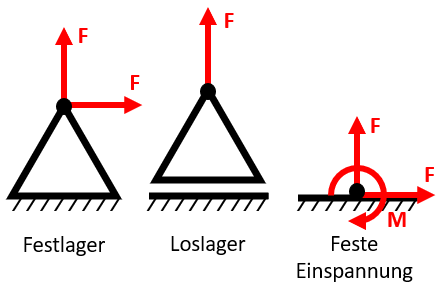
\includegraphics[width=0.3\textwidth]{Bilder/Einspannungen.png}
	\caption{Lagerarten mit ihren Freiheitsgradbeschränkungen (2D)}
\end{figure}
\begin{figure}[h]
	\centering
	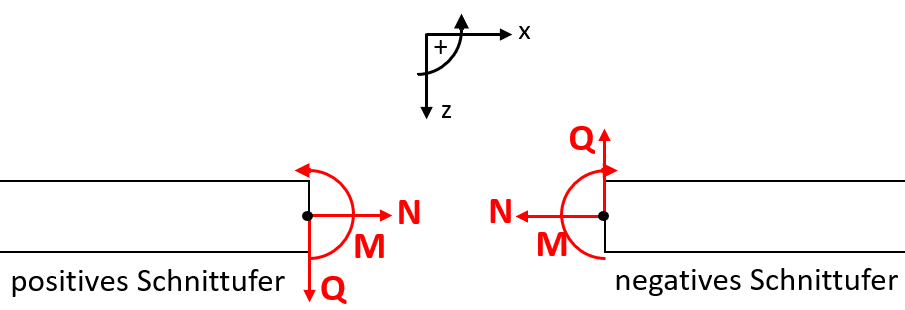
\includegraphics[width=0.7\textwidth]{Bilder/Schnittufer.png}
	\caption{Schnittkräfte und -momente in einem Balkenschnitt (2D)}
\end{figure}

\FloatBarrier
\newpage


\subsection{Einführung in die Netztheorie (H.G.)}
Bevor die klassische Laminattheorie entwickelt wurde, verwendete man die sogenannte Netztheorie. 
Bei der Netztheorie wird das Mittragen der Matrix vernachlässigt. Dadurch lassen sich die Schichtkräfte mit Hilfe eines Kräftegleichgewichts bestimmen. 
Durch diese Vereinfachungen kann der Konstrukteur schnell feststellen, ob die Fasern alleine der Belastung standhalten können. Wenn dies nicht der Fall ist werden die Kräfte größtenteils über die Matrix übertragen und das Laminat wird als \textit{ungesund} bezeichnet. Durch die Annahme, dass die Matrix nicht tragend ist, wird das Laminat jedoch unterschätzt und weist deutlich höhere Festigkeiten auf, als in der Netztheorie angenommen. Damit wird in jedem Fall eine Sicherheit mit eingerechnet.\\
Für die Verwendung der Netztheorie sollte das Gelege zunächst in ein Hauptachsenkoordinatensystem überführt werden, damit die Schubspannungen verschwinden. Die Kraftflüsse werden damit zu $\hat{n}_{I}$ und $\hat{n}_{II}$. Nun lässt sich der Winkel $\beta $ zwischen den Fasern und den Achsen des Hauptachsenkoordinatensystems bestimmen. Mit diesem und der Annahme, dass nur die Spannungen $\sigma_{\|}$ auftreten, können nun die Schnittkräfte in den Fasern bestimmt werden:
\begin{equation}
\hat{n}_{I}=\sum n_{\|k}\cdot cos^2\beta_{k}
\end{equation}
\begin{equation}
\hat{n}_{II}=\sum n_{\|k}\cdot sin^2\beta_{k}
\end{equation}
\begin{equation}
0=\frac{1}{2}\sum n_{\|k}\cdot sin2\beta_{k}.
\end{equation}
Da der gesamte Kraftfluss als Summe der Kraftflüsse in den einzelnen Fasern angenommen werden kann, lässt sich dadurch der Kraftfluss in den einzelnen Faserschichten und somit die benötigte Dicke der Schichten, bzw. die Anzahl der Lagen bestimmen\cite{item3}.

\noindent In der folgenden Berechnung wird die Netztheorie jedoch nicht verwendet, da die Auslegung vorerst mit der VDI 2013 erfolgt und anhand der Klassischen Laminattheorie.
\newpage
\subsection{Einführung in die Klassische Laminattheorie (H.G.)}\label{CLT}
Das Prinzip der klassischen Laminattheorie ist die Beschreibung des Elastizitätsgesetzes eines MSV durch die Elastizitätsgesetze der einzelnen Schichten. Dies lässt sich durch die Annahme eines ideal elastischen und fehlerfrei verklebten Mehrschichtverbund (MSV), wovon ein infinitesimales Scheibenelement betrachtet wird, realisieren. Zusätzlich gilt die Annahme, dass ein ebener Spannungszustand vorliegt, die Schnittspannungen über die Dicke konstant sind und keine Verwölbungen auftreten.\\
\noindent
Der Kraftfluss $\hat{n}$ im ganzen Laminat lässt sich durch die Summe der Kraftflüsse in den einzelnen Schichten zusammensetzen.
\begin{equation}
\label{Kraftfluss}
\hat{n}_{x}=\hat{\sigma}_{x}\cdot t=\sum n_{xk}=\sum\sigma_{xk}\cdot t_{k}
\end{equation}

\begin{equation}
\hat{n}_{y}=\hat{\sigma}_{y}\cdot t=\sum n_{yk}=\sum\sigma_{yk}\cdot t_{k}
\end{equation}

\begin{equation}
\hat{n}_{xy}=\hat{\tau}_{xy}\cdot t=\sum n_{xyk}=\sum\sigma_{xyk}\cdot t_{k}
\end{equation}
Nun lässt sich das Elastizitätsgesetz für den MSV aufstellen:
\begin{equation}
\label{Aep}
\lbrace \hat{n}\rbrace= [A]\cdot \lbrace\hat{\varepsilon}\rbrace .
\end{equation}
$[A]$ ist hierbei die Steifigkeitsmatrix des MSV. Mit Hilfe der Kraftfluss- Spannungsbeziehung aus Gleichung \ref{Kraftfluss}, lässt sich dann auf die Spannung schließen.
\begin{gather}
\begin{Bmatrix}
\hat{\sigma}_{x}\\
\hat{\sigma}_{y}\\
\hat{\tau}_{xy}\\
\end{Bmatrix}
=
\frac{1}{t}
\begin{bmatrix}
A_{11}&A_{12}&A_{16}\\
A_{12}&A_{22}&A_{26}\\
A_{16}&A_{26}&A_{66}
\end{bmatrix}
\cdot
\begin{Bmatrix}
\hat{\varepsilon}_{x}\\
\hat{\varepsilon}_{y}\\
\hat{\gamma}_{xy}\\
\end{Bmatrix}
\end{gather}
\noindent
Die Verzerrung des MSV und somit auch die Verzerrung der Einzelschichten, lässt sich nun durch die Umstellung von Gleichung \ref{Aep} bestimmen.
\begin{equation}
\label{SpannungDehnung}
\lbrace\hat{\varepsilon}\rbrace = [A]^{-1}\cdot\lbrace \hat{n}\rbrace
\end{equation}
\noindent
Um die Matrix A zu bestimmen werden die Steifigkeitsmatritzen der Einzelschichten $[Q]$ benötigt. Diese lassen sich mit Hilfe der E-Moduln, Querkontraktionszahlen definieren.
\begin{equation}
[Q]
=
\begin{bmatrix}
\frac{E_{\|}}{1-\nu_{\bot\|}\cdot \nu_{\|}\bot}&\frac{\nu_{\bot\|}\cdot E_{\bot}}{1-\nu_{\bot\|}\cdot \nu_{\|}\bot}&0\\
\frac{\nu_{\|\bot}\cdot E_{\|}}{1-\nu_{\bot\|}\cdot \nu_{\|}\bot}&\frac{E_{\bot}}{1-\nu_{\bot\|}\cdot \nu_{\|}\bot}&0\\
0&0&G_{\bot\|}
\end{bmatrix}
\end{equation}
\noindent
Da manche Faserschichten um einen Winkel $\alpha$ gedreht sein können, muss für diese Schichten die Steifigkeitsmatrix mit Hilfe der Transformationsmatrix $[T]$  nach der Transformationsregel aus Gleichung \ref{trafo} transforniert werden.
\begin{equation}
	\underline{\underline{T}}=
	\begin{bmatrix}
		\cos^{2}\alpha&\sin^{2}\alpha&-\sin 2\alpha\\
		\sin^{2}\alpha&\cos^{2}\alpha&\sin 2\alpha\\
		0,5\cdot \sin2\alpha&-0,5\cdot\sin2\alpha&\cos 2\alpha
	\end{bmatrix}
\end{equation}\\
\begin{equation}
\label{trafo}
	\overline{\underline{\underline{Q}}}=\underline{\underline{T}}\cdot \underline{\underline{Q}} \cdot \underline{\underline{T}}^{T}  
\end{equation}\\
\noindent
Nun lässt sich die Scheibensteifigkeits-Matrix [A] aus den Steifigkeitsmatritzen der einzelnen Schichten zusammensetzen (siehe Glg.\ref{AQ}).
\begin{equation}
\label{AQ}
	A_{ij}= \sum_{k=1}^{n} \overline{Q}_{ij,k}\cdot t_{k}
\end{equation}
\noindent
Um ein passende Anzahl an Faserschichten zu bekommen kann das Ergebnis nun iterativ angepasst werden.\cite{item3}
\subsubsection{Ingenieurskonstanten des MSV}
Für den einachsigen Spannungszustand lassen sich die Moduln und Querkontraktionszahlen für den MSV ableiten.
Diese lassen sich experimentell über z.B. einen Zugversuch oder rechnerisch aus dem Elastizitätsgesetz des MSV bestimmen.
\begin{equation}
\hat{E}_{x}=\frac{1}{A_{11}^{-1}\cdot t}
;
\hat{E}_{y}=\frac{1}{A_{22}^{-1}\cdot t}
;
\hat{G}_{xy}=\frac{1}{A_{66}^{-1}\cdot t}
;
\hat{\nu}_{xy}=-\frac{A_{12}^{-1}}{A_{22}^{-1}}
;
\hat{\nu}_{yx}=-\frac{A_{12}^{-1}}{A_{11}^{-1}}
\end{equation}
\noindent
Die Spannungen lassen sich jetzt durch Gleichung \ref{SpannungDehnung} errechnen.\\
\noindent
Bei den Elastizitätsmoduln ist darauf zu achten, dass es sich um Moduln ohne Querkontraktionsbehinderung handelt \cite{item3}.
\subsubsection{Plattenelement}
Um ein Plattenelement zu Berechnen werden zusätzliche Beziehungen benötigt, da nun ein zweiachsiger Spannungszustand vorliegt. Zu Gleichung \ref{AQ} kommen nun noch 2 weitere Gleichungen (siehe Glg.\ref{BQ}/\ref{DQ}) hinzu. $|z_{k}|$ ist der Abstand zwischen den Schichten.
\begin{equation}
\label{BQ}
	B_{ij}= \cdot \sum_{k=1}^{n} \overline{Q}_{ij,k}\cdot t_{k}\cdot \left(z_{k}-\frac{t_{k}}{2}\right)
\end{equation}
\begin{equation}
\label{DQ} 
	D_{ij}=\sum_{k=1}^{n} \overline{Q}_{ij,k}\cdot \left(\frac{t_{k}^{3}}{12}+t_{k}\left(z_{k}-\frac{t_{k}}{2}\right)^{2}\right)
\end{equation}
\noindent
Nun lässt sich die Scheiben-Platten-Beziehung als Gleichung \ref{S-P} schreiben.\cite{item3}
\begin{equation}
\label{S-P}
	\begin{pmatrix}
		\hat{\underline{n}}\\
		\hat{\underline{m}}
	\end{pmatrix}
	= \begin{bmatrix}
		\underline{\underline{A}}&\underline{\underline{B}}\\
		\underline{\underline{B}}&\underline{\underline{D}}
	\end{bmatrix}
	\cdot \begin{pmatrix}
		\underline{\epsilon}\\
		\underline{\kappa}
	\end{pmatrix}
\end{equation}\\


\newpage
\subsection{Einführung in die Mischungsregel (H.G.)}
Um die Materialkonstanten des FKV zu ermitteln kann die Mischungsregel verwendet werden. Darin werden die Materialkonstanten der Fasern und der Matrix im Verhältnis zu ihrem Massenanteil zu einer FKV-Materialkonstante zusammengestellt.\\
\noindent
Die Dichte des FKV lässt sich aus der Dichte der einzelnen Komponenten errechnen (siehe Glg. \ref{dichte}).
\begin{equation}
\label{dichte}
	\rho=\rho_{F}\cdot\varphi +\rho_{M}\cdot (1-\varphi)
\end{equation}
\noindent
Der E-Modul parallel (siehe Glg. \ref{Eparallel}) und orthogonal (siehe Glg. \ref{Eorthogonal}) kann mit den E-Modulen von Faser und Matrix, sowie dem Faservolumenanteil $\varphi$ errechnet werden. Zu betonen ist hierbei, dass auf eine Querkontraktionsbehinderung der Matrix durch die Fasern nicht eingegangen wird. In diesem Fall wären die resultierenden Steifigkeiten größer. Um sicher konservativ rechnen zu können, wird demnach die vereinfachte Rechnung benutzt. Aus selbigem Grund wird daher auch auf höhere Mischungsregeln, wie z.B. nach Puck, verzichtet. 
\begin{equation}
\label{Eparallel}
E_{\|}=E_{f\|}\cdot \varphi+E_{m}\cdot (1-\varphi)
\end{equation}

\begin{equation}
\label{Eorthogonal}
E_{\bot}=\frac{E_{m}}{(1-\varphi)\cdot\frac{E_{m}}{E_{f\bot}}\cdot\varphi}
\end{equation}
\noindent
Der Schubmodul in Faser-Quer-Längs-Richtung kann ebenfalls durch die Schubmodule der Fasern und der Matrix ermittelt werden.
\begin{equation}
G_{\bot\|}=G_{m}\frac{1}{(1-\varphi)+\frac{G_{m}}{G_{f\bot\|}}\cdot\varphi}
\end{equation}
Außerdem lassen sich die Querkontraktionszahlen berechnen.
\begin{equation}
\nu_{\bot\|}=\varphi\cdot \nu_{f\bot\|}+(1-\varphi)\cdot \nu_{m}
\end{equation}
Aus diesen Werten lassen sich alle weiteren durch die Beziehungen zwischen den Materialkonstanten berechnen.\cite{item3}
\newpage
\subsection{Einführung in das Versagenskriterium nach Puck (O.S.)}
Da für einen anisotropen FKV nicht das Versagen mittels einer allgemeinen resultierenden Spannung für jeden Lastfall ermittelt werden kann, müssen Versagenskriterien für die speziellen Beanspruchungsmodi definiert werden. Für die in dieser Projektarbeit durchgeführten Auslegungen wurden die Festigkeitskriterien von Puck verwendet. Hierbei werden die einzelnen UD-Schichten des Laminats getrennt betrachtet. Auch wenn diese Betrachtungen physikalisch begründet sind (vgl. \cite{EdL}), hat dies zur Folge, dass Effekte wie Delamination nicht berücksichtigt werden.
\subsubsection{Definitionen}
Zunächst sind einige Begriffe zu definieren. An einer UD-Schicht können zwei verschiedene Normalspannungen wirken, die sich, je nachdem, ob es sich um Druck- oder Zugbelastung handelt, unterschiedlich auf das Versagen auswirken: die Längsbeanspruchung $\sigma_{\parallel}$ parallel und die Querbeanspruchung $\sigma_{\perp}$ orthogonal zur Faserrichtung. Auch bei der Schubspannung muss zwischen der Quer-/Quer-Schubbeanspruchung $\tau_{\perp\perp}$ und der Längs-/Quer-Schubbeanspruchung $\tau_{\parallel\perp}$ unterschieden werden. Wegen des durch die Fasern bedingten stark anisotropen Aufbaus muss zwischen zwei grundlegenden Versagensarten unterschieden werden: dem Faserbruch (Fb) und dem Zwischenfaserbruch (Zfb). Der Begriff Bruch ist hier bewusst als Schadensbezeichnung gewählt, da bei beiden Fällen kein plastisches Verhalten auftritt und es sich um einen Sprödbruch ohne nennenswertes Fließen handelt.
Für das Versagenskriterium wird die genaue Definition der Anstrengung $f_E$ gesucht. Diese ist abhängig vom Spannungszustand und immer so definiert, dass bei $f_E=1$ das Versagen eintritt, sie also bei Belastungen, die das Material, aushält Werte kleiner als $1$ und bei überkritischen Lasten größer $1$ annimmt.

\noindent Beim Zfb stimmt die Bruchebene nicht unbedingt mit der Wirkebene, der Ebene mit der höchsten Beanspruchung, überein. Auf anderen Ebenen können andere Festigkeiten herrschen, die früher überschritten werden. Generell gilt für sie, dass die Bruchebene immer parallel zu den Fasern sein muss. Puck führt analog zur Festigkeit den Bruchwiderstand der Wirkebene $R^A$, der als "derjenige Widerstand [definiert ist], den eine Schnittebene ihrem Bruch infolge einer einzelnen in ihr wirkenden Beanspruchung (bei Zfb: $\sigma_\perp^+$ oder $\tau_{\perp\perp}$ oder $\tau_{\parallel\perp}$) entgegensetzt"\cite{item3}.
\subsubsection{Zwischenfaserbruch ohne Längsspannung}
Ignoriert man die Längsspannung $\sigma_1$, da diese erst bei sehr hohen Werten Einfluss auf einen Zfb hat, ergibt sich ein Spannungszustand aus den beiden übrigen Normalspannungen $\sigma_2$ und $\sigma_3$ orthogonal zu den Fasern und den Schubspannungen $\tau_{12}$, $\tau_{23}$ und $\tau_{31}$. Um nun die Bruchebene bestimmen zu können, muss der Spannungszustand in dieser Ebene mittels der Matrix aus Gleichung \ref{Bruchebene} transformiert werden. Aus der Bedingung, dass die Bruchebene parallel zu den Fasern liegen muss, ergibt sich eine Drehung um die $x_1$-Achse, die in Faserrichtung zeigt, mit dem Winkel $\theta$. In der Bruchebene liegen dann nur noch die beiden Schubspannungen $\tau_{nt}$ normal und tangential zur Ebene, $\tau_{n1}$ normal in Faserrichtung und die Normalspannung $\sigma_n$ senkrecht auf der Bruchebene.
\begin{equation}\label{Bruchebene}
	\begin{pmatrix}
		\sigma_n \\ \tau_{nt} \\ \tau_{n1}
	\end{pmatrix}
	=
	\begin{pmatrix}
		c^2 & s^2 & 2cs & 0 & 0\\
		-cs & sc & (c^2-s^2) & 0 & 0\\
		0 & 0 & 0 & s & c
	\end{pmatrix}
	\cdot
	\begin{pmatrix}
		\sigma_2 \\ \sigma_3 \\ \tau_{23} \\ \tau_{31} \\ \tau_{12}
	\end{pmatrix}
\end{equation}
Mit
\begin{equation}
	c = cos\theta
\end{equation}
und
\begin{equation}
	s = sin\theta.
\end{equation}
%Die Schubspannungen lassen sich des Weiteren zu einer Resultierenden 
%\begin{equation}
%	\tau_{n\psi} = \sqrt{\tau_{nt}^2 + \tau_{n1}^2}
%\end{equation}
%zusammenfassen.
Mit diesen Werten definiert Puck seine Bruchbedingungen aus der Mohrschen Bruchhypothese\cite{item3}, wobei er zwischen $\sigma_n < 0$:
\begin{equation}\label{Zfb1}
	f_{E,\mathrm{Zfb}} = \sqrt{\biggl[\biggl(\frac{1}{R_{\perp}^+}-\frac{p_{\perp\psi}^+}{R_{\perp\psi}^A}\biggl)\sigma_n\biggl]^2 + \biggl(\frac{\tau_{nt}}{R_{\perp\perp}^A}\biggr)^2 + \biggl(\frac{\tau_{n1}}{R_{\perp\parallel}}\biggr)^2} +  \frac{p_{\perp\psi}^+}{R_{\perp\psi}^A}\sigma_n
\end{equation}
und $\sigma_n \geq 0$
\begin{equation}\label{Zfb2}
	f_{E,\mathrm{Zfb}} = \sqrt{\biggl(\frac{p_{\perp\psi}^-}{R_{\perp\psi}^A}\sigma_n\biggr)^2 + \biggl(\frac{\tau_{nt}}{R_{\perp\perp}^A}\biggr)^2 + \biggl(\frac{\tau_{n1}}{R_{\perp\parallel}}\biggr)^2} +  \frac{p_{\perp\psi}^-}{R_{\perp\psi}^A}\sigma_n
\end{equation}
unterscheidet. Mit den experimentell ermittelten Bruchwiderständen $R$ und Steigungsparametern $p_{\perp\perp}^\pm$ lassen sich aus der Bedingung, dass der Bruchkörper, welcher sich aus $f_{E,\mathrm{Zfb}} = 1$ ergibt, sprung- und knickfrei sein muss, somit die Neigungsparapameter $p_{\perp\psi}^\pm$ bestimmen. Nun lässt sich die Anstrengung in Abhängigkeit des Drehwinkels $\theta$ errechnen. Für die meisten Fälle ist dies jedoch nicht analytisch möglich, sodass die Werte numerisch bestimmt werden müssen. In der Ebene mit der höchsten Anstrengung kann es am ehesten zum Bruch kommen. Der Reservefaktor ist als der Kehrwert der Anstrengung definiert und ist ein Maß für die Sicherheit gegen das Versagen. Falls die Anstrengung den Wert von $1$ überschreitet, wird die Ebene der UD-Schicht zur Bruchebene, wo der Reservefaktor zuerst null wird. Es kommt zum Zwischenfaserbruch.
\subsubsection{Einfluss der Längsspannung}
In diesen Betrachtungen wurde bisher der Einfluss der Spannung in Faserrichtung $\sigma_1$ vernachlässigt. Jedoch treten bei höheren Spannungen Effekte auf, die sich auch auf den Zfb auswirken und die Bruchwiderstände senken. Zum einen wird durch starke Dehnung in Faserrichtung die Matrix überproportional beansprucht und Poren werden verstärkt geöffnet, zum anderen kann es auch, bevor Faserbruch eintritt, zum Bruch einzelner Filamente kommen, die Risse in der Matrix begünstigen. Außerdem können sich durch Druckspannungen in Faserrichtung leicht wellen, was zusätzliche $\tau_{\perp\parallel}$-Beanspruchung in das Material einträgt.

\noindent Puck berücksichtigt diese Senkung der Bruchwiderstände durch einen Schwächungsfaktor $\eta_\mathrm{w} < 1$. Um die Einbeziehung dieses Faktors besser handhabbar zu machen, wird er für alle Bruchwiderstände gleich gewählt. Somit lässt er sich sowohl aus Gleichung \ref{Zfb1}, als auch \ref{Zfb2} ausklammern. Es lässt sich also die Bruchbedingung unter Einbezug der Längsspannung $f_{E1} = 1$ als
\begin{equation}
	f_{E1} = \frac{f_{E0}}{\eta_\mathrm{W}} = 1
\end{equation}
schreiben, wobei der Index 0 für die Anstrengung ohne $\sigma_1$ steht. Durch die gleich starke Absenkung aller Bruchwiderstände bleibt auch der Bruchwinkel erhalten. Für die Abhängigkeit des Schwächungsfaktors von $\sigma_1$ wird eine Ellipsenbeziehung gewählt, wobei wieder zwischen Druck- und Zugspannung unterschieden wird, da die Zugspannung einen stärkeren Einfluss auf den Zfb hat. Dadurch ergibt sich für den Bruchkörper eine Zigarrenform.

\noindent Auch wenn Zwischenfaserbrüche nicht unbedingt zum Totalversagen des Laminats führen, sind sie hier trotzdem als Auslegungskriterium zu sehen, da sie negative Auswirkungen auf die Festigkeiten, Lebensdauer und Sicherheit haben. Die Risse in der Matrix können Delamination auslösen oder auch durch Kerbwirkung anliegende Schichten schwächen. Sowohl der Quer-Längs-Schubmodul als auch die Bruchfestigkeit $R_\parallel^-$ nehmen ab. Des Weiteren können durch die Risse korrosive Medien an die Fasern gelangen und diese schädigen.
\subsubsection{Faserbruch}
Ein viel kritischerer Fall tritt ein, wenn beim Faserbruch die Fasern reißen oder brechen. Als Versagen gilt hier nicht der Bruch einzelner Fasern, sondern ganzer Bündel. Dies ist unter allen Umständen zu vermeiden, da die hohen Spannungen, bei denen das Material versagt, meist nicht über andere Lastpfade kompensiert werden können. Während die Spannung in Faserrichtung $\sigma_{\parallel}$ für den Zfb nur eine zweitrangige Rolle spielt, ist sie für den Fb maßgebend.
\paragraph{Zugspannung $\sigma_{\parallel}^+$}~\\
Der Bruchwiderstand in Faserrichtung bei Zugbeanspruchung $R_\parallel^+$ wird in der Regel rechnerisch und nicht experimentell bestimmt. Der genaue Wert für die Festigkeit wird meistens nicht benötigt, weil bei FKV viel schneller durchs Versagen der Matrix ein Zfb auftreten kann und die Konstruktionen bei schwingender Beanspruchung durch Ermüdung versagen. Außerdem ist die Bestimmung des Wertes im Versuch möglich, weil es wegen der hohen Bruchspannungen an den Einspannungen zu mehrachsigen Spannungszuständen kommt. Da die Fasern quasi die gesamte Spannung aufnehmen und die Matrix dem gegenüber vernachlässigbar ist, lässt sich die Festigkeit des Laminats rein aus der der Fasern $R_{f \parallel}^+$ und des Faservolumenanteils $\varphi$ bestimmen:
\begin{equation}
	R_\parallel^+ = R_{f \parallel}^+\varphi
\end{equation}
Hieran lässt sich auch erkennen, dass die Spannungen, die in den Fasern herrschen, antiproportional mit dem Faservolumenanteil steigen. Jedoch kann man diesen Wert nicht ohne weiteres verwenden, sondern muss ihn durch einen Abminderungsfaktor korrigieren, da die wahre Festigkeit durch einige Effekte gesenkt wird.

\noindent Schon in der Fertigung und Verarbeitung können Schädigungen an einzelnen Filamenten entstehen, sodass diese früher versagen und benachbarte Fasern einer erhöhten Belastung ausgesetzt sind. Auch eine leicht unterschiedliche Ausrichtung oder Vorspannung kann zu einer unterschiedlichen Spannungsverteilung führen, die das vorzeitige Versagen bewirkt. Die örtliche Streuung der Festigkeit sorgt dafür, dass einige Fasern zuerst brechen und anliegende ihr Last zusätzlich tragen müssen. Auch wenn dadurch die Gesamtfestigkeit des FKVs gesenkt wird, ermöglicht dies das vorzeitige Erkennen des Versagens, was erwünscht ist.
\paragraph{Druckspannung $\sigma_{\parallel}^-$}~\\
Bei hohen Druckspannungen, besonders bei dünnen Bauteilen des Leichtbaus, muss es nicht zum Versagen des Materials in Folge vom Erreichen der Fließgrenze oder Schubbelastung spröder Werkstoffe kommen. Es handelt sich stattdessen um ein Stabilitätsproblem, bei dem die Fasern einer UD-Schicht knicken. Jedoch kommt es nur in einem nie wirklich erreichbaren idealen Laminat zu einem Verzweigungsproblem, wie es beim Eulerknicken zu beobachten ist. Bei realen Laminaten gibt es immer Imperfektionen, bei denen die Fasern durch Welligkeiten lokal eine variierende Orientierung haben, die das sogenannte Schubknicken auslösen.
\begin{figure}
	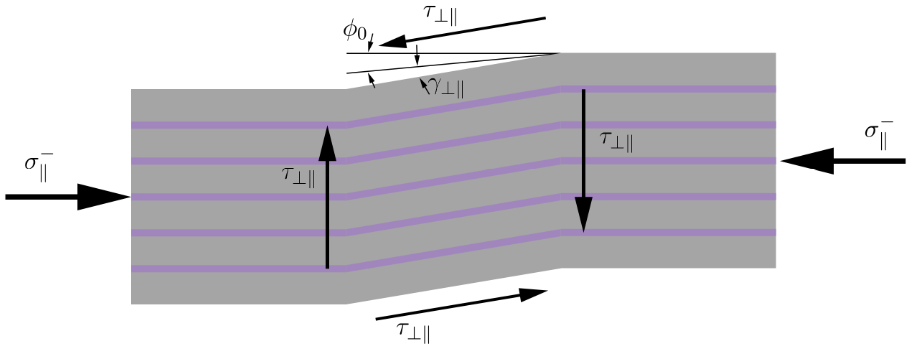
\includegraphics[width=1.0\textwidth]{Bilder/Schubknicken.png}
	\caption{Kräfte beim Schubknicken von VFK}
	\label{fig:Schubknicken}
\end{figure} 
Schon ohne Lastangriff liegt also eine Orientierungsabweichung mit dem Winkel $\phi_0$ vor. Da trotzdem an jeder Stelle das Momentengleichgewicht herrschen muss, aber es an diesem Ort nicht mehr nur durch die Druckspannungen erfüllt ist, entstehen Schubspannungen $\tau_{\perp\parallel}$. Aus dem Momentengleichgewicht in Abbildung \ref{fig:Schubknicken} lässt sich der Zusammenhang
\begin{equation}\label{SchubknickSigma}
	\sigma_{\parallel}^-=\frac{\tau_{\perp\parallel}}{\phi_0 + \gamma_{\perp\parallel}}
\end{equation}
erkennen. Mit steigender Druckspannung steigt auch der Schiebewinkel $\gamma_{\perp\parallel}$. Bei dieser Betrachtung wurde aber noch die Biegesteifigkeit der Fasern außer Acht gelassen, die dem Schubknicken entgegenwirken. Auch die benachbarten Fasern stützen die knickenden Schichten und tragen somit zu einer erhöhten Stabilität bei. Des Weiteren ist zu beachten, dass die Schubspannung $\tau_{\perp\parallel}$ stark nichtlinear von dem Schubwinkel $\gamma_{\perp\parallel}$ abhängt. 
Die Längs-Druckfestigkeit $R_\parallel^-$ lässt sich aus der Extremwertbetrachtung von Gleichung \ref{SchubknickSigma} als der Maximalwert von $\sigma_{\parallel}^-$ zu
\begin{equation}
	R_\parallel^- = \frac{\mathrm{d}\tau_{\perp\parallel}}{\mathrm{d}\gamma_{\perp\parallel}} = G_{\perp\parallel,\mathrm{T}}(\gamma_{\perp\parallel})
\end{equation}
bestimmen. $G_{\perp\parallel,\mathrm{T}}(\gamma_{\perp\parallel})$ ist der Tangenten-Schubmodul beim Schubknicken. Wird dieser Wert überschritten, wächst der Schiebewinkel unkontrolliert an und es kommt zum lokalen Knicken, was nicht selten zum Gesamtversagen führen kann.

\noindent Häufig kommt es aber gar nicht zur Überschreitung dieser Festigkeit. Lokale Spannungsmaxima können schon vorher zum Versagen durch Zfb führen, bevor es zum Schubknicken kommt. In dem zu konstruierenden Flügel soll sich ein Holm befinden, in dessen Gurten es durch ihre relativ hohe Dicke jedoch trotzdem vorkommen kann. Somit ist dieser Fall für diese Projektarbeit nicht vernachlässigbar.

\noindent Sowohl die Längs-Druckfestigkeit $R_\parallel^-$ als auch die Längs-Zugfestigkeit $R_\parallel^+$ sind als Materialkennwerte der UD-Schicht im Rahmen der Aufgabenstellung gegeben und ergänzen die Pucksche Zigarre, indem der Bruchkörper durch diese beiden Festigkeiten in die $\sigma_1$-Richtung beschränkt wird.
\begin{figure}[h]
	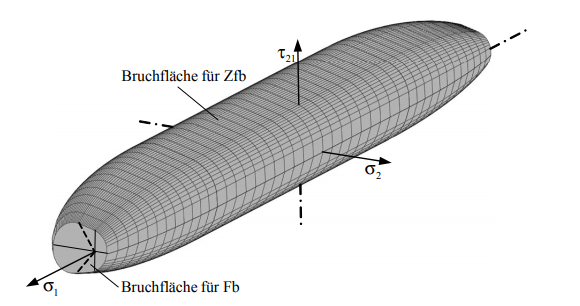
\includegraphics[width=1.0\textwidth]{Bilder/Zigarre.png}
	\caption{Pucksche Zigarre aus \cite{item3}}
\end{figure} 
\newpage
\FloatBarrier
\:
\newpage
\subsection{Einführung in Stabilitäts-Überprüfungen (T.B.)}\label{Beulen}
Neben der Festigkeit und Steifigkeit ist es bei einer Konstruktion dünnwandiger Bauteile notwendig, sie auf Versagen durch mangelnde statische Stabilität zu überprüfen. Stabilität bedeutet, dass ein System bestimmte maximale Lasten erträgt, es bei schon kleinen Erhöhungen jedoch zu drastischen Systemänderungen, wie z.B. in der Tragfähigkeit, kommen wird. Bemerkbar ist dieses auch in Veränderungen der Bauteilgeometrie \cite{item16}.\\

\noindent Typische Versagensarten aufgrund zu hoher Druckbeanspruchungen bilden dabei das Knicken (eindimensionale Formänderung) und das Beulen (zweidimensionale Formänderung). Bei Letzterem haben auch Schubbeanspruchungen Einfluss darauf. Dabei entstehen wellenförmige Ausprägungen des Bauteils (in entsprechend vielen Dimensionen). Sie können mit unendlich vielen Eigenwerten beliebig viele Ausprägungen, einer Sinus-Funktion mit unterschiedlichen Frequenzen entsprechend, im Bauteil bilden. Die kritische Last wird für eine einfache Ausprägung definiert, da dieser Fall zuerst eintreten wird. Die Verformungen können auch plastisch auftreten, sodass nach Entlastung des Bauteils irreparable Schäden bleiben. Inwiefern ein Bauteil im geknickten bzw. gebeulten Zustand seine Eigenschaften beibehält, lässt sich kaum vorhersagen \cite{item16}.\\

\noindent Die Beulsicherheit der Tragflügel-Bauteile erfolgt nach Hertel \cite{item1}. Dabei handelt es sich um Theorien isotroper Stoffe. Dennoch werden sie hier für FVK angewendet, da im Orthotropie-Achsensystem gleiche Verhaltensweisen wie isotroper Stoffe gelten. Die Orthotropie ist in nachfolgenden Bauteilen hinreichend durch gewählte Belastungsrichtungen und Lagenaufbauten gegeben (siehe Kapitel 4 und 5). Diese Annahme hat sich bei bisherigen Flugzeug-Konstruktionen und deren Zulassungen bewährt \cite{item21}.\\

\noindent In der Hautebene eines dünnwandigen Bauteils wird zwischen beulkritischen Spannungen unterschieden, die aus reiner Biegung, Druck und Biegung, oder reinem Schub (Indizes $b$/$d$/$s$) resultieren. Sofern Normal- und Schubspannungen gleichzeitig vorliegen, kann lediglich eine kombinierte Belastung als über- oder unterkritisch eingestuft werden. Die Spannungen und Beulausprägungen sind von folgenden Parametern abhängig \cite{item1}:
\begin{itemize}
	\item Seitenverhältnis $\frac{a}{b}$. Für einen Betrag gleich Null wird das Hautfeld \glqq Streifen\grqq\: genannt. 
	\item Randbedingungen an den Rändern des Hautfelds. Ränder können frei (alle Freiheitsgrade), gestützt (rotatorischer Freiheitsgrade) und fest (keine Freiheitsgrade )gelagert werden.
	\item relative Hautstärke $\frac{s}{b}$.
	\item Elastizitätsmodul $E$.
\end{itemize}
Dabei stehen $a$ und $b$ für die lange bzw. die kurze Seite des Hautfelds und $s$ für dessen Hautstärke. Mit dem Seitenverhältnis und den Randbedingungen ergibt sich ein Beulfaktor $k$, der, je nach vorherrschender Beanspruchung, in den Abbildungen \ref{fig: Hertel_Druck}, \ref{fig: Hertel_Biegung} und \ref{fig: Hertel_Schub}  ermittelt wird. \\
Die beulkritischen Normal- und Schubspannungen lassen sich nach
\begin{equation}
	\sigma_{krit}=k\cdot E\cdot\Big(\frac{s}{b}\Big)^{2}
\end{equation}
\begin{equation}
	\tau_{krit}=k\cdot E\cdot\Big(\frac{s}{b}\Big)^{2}
\end{equation}
berechnen. Die Sicherheit gegen Beulen ergibt sich aus dem Verhältnis zur tatsächlich anliegenden Spannung $\sigma_{max}$ bzw. $\tau_{max}$. Falls beide Spannungstypen gleichzeitig anliegen sollten, kann mit der Gleichung
\begin{equation}
	\Big(\frac{\tau}{\tau_{krit}}\Big)^{2}+\Big(\frac{\sigma}{\sigma_{krit}}\Big)^{2}=1^{2}=j^{2}
\end{equation}
in Abbildung \ref{fig: Hertel_Sicherheit} herausgefunden werden, ob es sich um einen überkritischen Zustand handelt \cite{item1}.\\

\noindent Generell werden Krümmungen und Versteifungen nachfolgend vernachlässigt. Allerdings sind für Sandwich-Bauteile Anpassungen durchzuführen:\\
Die Dicke $d$ beinhaltet neben den FVK-Lagen die Schaumstoffdicke. Dadurch, dass diese Lagen nun an den Außenseiten konzentriert sind, kann das Trägheitsmoment mit einem Faktor $\kappa$ bis auf das Dreifache maximal erhöht werden. Dieser wird jedoch wieder minimiert, sofern der Lagenaufbau unsymmetrisch und somit das Dickenverhältnis ungleich eins ist. Exakte Beträge können der Abbildung \ref{fig: Hertel_Sandwich} entnommen werden. Die beulkritischen Spannungen berechnen sich somit nach \cite{item1} zu
\begin{equation}
	\sigma_{krit}=\kappa\cdot k\cdot E\cdot\Big(\frac{d}{b}\Big)^{2}
\end{equation}
\begin{equation}
	\tau_{krit}=\kappa\cdot k\cdot E\cdot\Big(\frac{d}{b}\Big)^{2}
\end{equation}
\newpage

\subsection{Einführung in den Kraftfluss dünnwandiger Profile (O.S.)}\label{Trägheitsmomente}
Im Leichtbau ist es wichtig geeignete Konstruktionen zu entwerfen, um Eigenschaften der Werkstoffe ideal nutzen zu können. Das Gesamtbauteil ist dann meist so kompliziert, dass sich die für das Bauteil zu lösenden Differenzialgleichungen, wie zum Beispiel die der Elastostatik, keine geschlossenen Lösungen finden lassen. Das Ziel ist es nun durch Annahmen und Vereinfachungen ein sinnvolles und lösbares Ingenieursmodell zu finden. Alternativ könnten auch Lösungen mittels numerischer Methoden ermittelt werde, hierzu mehr in Kapitel \ref{FEM-Theorie}.

\paragraph{Zylindrische, dünnwandige Profile}~\\
Häufig werden zylindrische, dünnwandige Profil genutzt, da sie bei vergleichsweiser niedriger Masse noch immer gute Werte bei zum Beispiel der Biegesteifigkeit liefern. Sie zeichnen sich dadurch aus, dass sie deutlich höhere Ausmaße in x-Richtung haben, als in jede andere (zylindrisch). Eine Laufvariable $s$ verläuft in der y-z-Ebene durch die Mitte der Profildicke $t(s)$. Die Dicke ist nicht zwangsläufig über $s$ konstant, muss aber deutlich kleiner als alle anderen Abmessungen sein (dünnwandig) \cite{item15}. Man kann vereinfacht annehmen
\begin{equation}
	\iint dA=\int t(s)ds.
\end{equation} 
Der Querschnitt muss in x-Richtung konstant sein und auch bei Belastung seine Gestalt beibehalten. Der Schubfluss im Profil ist als
\begin{equation}\label{tau}
	q=\tau t(s)
\end{equation}
und der Normalkraftfluss als
\begin{equation}
	n_x=\sigma_x t(s)
\end{equation}
definiert. Für diese Kraftflüsse gilt das hydrodynamische Analogon. Das heißt, mit einer Änderung der Dicke muss der Kraftfluss antiproportional ab- bzw. zunehmen, damit das Kräftegleichgewicht erfüllt bleibt. Für Knotenpunkte muss auch gelten, dass der Betrag der Kraftflüsse in den Knoten hinein denen aus ihm heraus gleicht. Des Weiteren lässt sich noch zwischen offenen und geschlossenen Profilen unterscheiden, wobei es sich bei zweiterem um Ein- oder Mehrzeller handeln kann \cite{item15}.

\paragraph{Koordinatensysteme}~\\
Bei den Berechnungen kann viel Arbeit gespart werden, indem das Koordinatensystem mit Ursprung und Achsenausrichtung klug gewählt wird. Das allgemeine Koordinatensystem, das unabhängig vom betrachteten Profil ist, bietet hierbei die wenigsten, wenn nicht sogar keine Vorteile. Verschiebt man seinen Ursprung in den Schwerpunkt, erhält man das Schwerpunkt-Koordinatensystem. Es wird mit einem Querstrich über den Koordinaten gekennzeichnet ($\bar{x},\bar{y},\bar{z}$). Es ist sinnvoll aus dieser Perspektive den Schubfluss zu betrachten.
\begin{figure}[h]
	\centering
	\includegraphics[width=1\textwidth]{Bilder/schubfluss-infinit}
	\caption{Infinitesimales Profilelement aus \cite{item15}}
	\label{schubfluss-infinit}
\end{figure}
Aus dem Kräftegleichgewicht in $x$- und $s$-Richtung an einem infinitesimalen Volumen des dünnwandigen Profils ergibt sich der Zusammenhang zwischen den Kraftflüssen zu
\begin{equation}
	\frac{\partial n_x}{\partial x} + \frac{\partial q}{\partial s} = 0
\end{equation}
\begin{equation}\label{n_s}
	\frac{\partial n_s}{\partial s} + \frac{\partial q}{\partial x} = 0
\end{equation}
Da jedoch eine Krümmung in $s$-Richtung vorliegen kann, zeigt die Resultierende des Normalkraftflusses $n_s$ aus der Ebene heraus. Da bei dünnen Scheibenelementen ein ebener Spannungszustand herrscht, darf dies nicht sein. Daraus folgt, dass beide Terme in Gleichung \ref{n_s} gleich null sein müssen. Der Schubfluss ist also in $x$-Richtung konstant und lässt sich somit zu
\begin{equation}
	q(s)=-\int\frac{\partial n_x(x,s)}{\partial x}ds+q_0.
\end{equation}
integrieren. Wird nun der Normalkraftfluss in Abhängigkeit von der Querkraft $Q$ gesetzt, ergibt sich die $Q$-$SI$nen-Formel nach \cite{item15}:
\begin{equation}\label{qs}
	q(s)=-(Q_{\bar{z}}\frac{S_{\bar{y}}(s)I_{\bar{z}}-S_{\bar{z}}(s)I_{\bar{yz}}}{I_{\bar{y}}I_{\bar{z}}-I_{\bar{yz}}^2}+Q_{\bar{y}}\frac{S_{\bar{z}}(s)I_{\bar{y}}-S_{\bar{y}}(s)I_{\bar{yz}}}{I_{\bar{z}}I_{\bar{y}}-I_{\bar{yz}}^2})+q_0
\end{equation}
mit den Flächenträgheitsmomenten
\begin{equation}\label{FT1}
	I_{y} = \int_{A}^{}z^2dA ~\ ,
\end{equation}
\begin{equation}
	I_{z} = \int_{A}^{}y^2dA
\end{equation}
und
\begin{equation}\label{FT3}
	I_{yz} = \int_{A}^{}zydA  ~\ .
\end{equation} 
Spätestens hier zeigt sich, dass für dieses Modell das Superpositionsprinzip anwendbar ist und man die Kräfte $Q_y$ und $Q_z$ getrennt betrachten kann.
Hier lässt sich direkt erkennen, wie diese Formel durch die Wahl eines besseren Koordinatensystems vereinfacht werden kann. Für das Hauptachsen-Koordinatensystem bleibt der Schwerpunkt weiterhin der Ursprung, jedoch werden die Achsen so um die x-Achse gedreht, dass die Deviationsmomente $I_{yz}$ verschwinden. Es wird mit einem Dach über den Koordinaten gekennzeichnet ($\hat{x},\hat{y},\hat{z}$). Die Integrationskonstante
\begin{equation}
	q_{0} = q_{0b}+q_{0T}
\end{equation}
ist nur bei geschlossenen Profilen ungleich null. Sie sich aus einem Teil, der aus der Biegung entsteht, $q_{0b}$, und einem aus der Torsion, $q_{0T}$, zusammen. Es gibt einen Punkt in der y-z-Ebene für jedes Profil, wo eine angreifende Kraft keine Torsion verursacht. Dieser Punkt ist von hoher Bedeutung und wird Schubmittelpunkt genannt.
\newpage
\subsection{Einführung in die Finite Elemente Methode (O.S.)}\label{FEM-Theorie}
\subsubsection{Schwache Lösung der Elastostatik}
Für die Berechnung der Elastostatik sind die Gleichgewichtsbedingung (\ref{GGB}),  Verzerrungs-Verschiebungsbedingung (\ref{VVB}) und das Stoffgesetz (\ref{SG}) auch bei der Finiten Elemente Methode (FEM) ausschlaggebend
\begin{equation}\label{GGB}
	\underline{0} = \underline{X} + \underline{\underline{D}}^T \sigma 
\end{equation}
\begin{equation}\label{VVB}
	\underline{\epsilon} = \underline{\underline{D}} \underline{u}
\end{equation}
\begin{equation}\label{SG}
	\underline{\sigma} = \underline{\underline{E}} \underline{\epsilon}
\end{equation}
\cite{item14}. Wobei \underline{$X$} der Vektor der Volumenkräfte, \underline{\underline{$E$}} die Steifigkeitsmatrix, \underline{$\epsilon$} der Verzerrungsvektor, \underline{$u$} der Verschiebungsvektor und \underline{\underline{$D$}} die Operatormatrix ist.\\
Um einer aufwendigen Bestimmung der analytischen Lösung zu entgehen, bedient sich die FEM dem Prinzip der \textit{schwachen Lösung}. Hierbei hat man eine Differenzialgleichung, die in dem betrachteten Gebiet gleich null ist. Für die Elastostatik kann man hierbei die Gleichgewichtsbedingung verwenden. Diese kann man mit der virtuellen Verschiebung $\delta\underline{u}$ multiplizieren und über das Gebiet integrieren, sodass man
\begin{equation}
	\int_{V}^{}\delta\underline{u}^T\underline{\underline{D}}^T\underline{\sigma}\,dV + \int_{V}^{}\delta\underline{u}^T\underline{X}\,dV = 0
\end{equation}
erhält. Umgeformt ergibt sich das zu
\begin{equation}\label{SL}
	\int_{V}^{}\delta\underline{u}^T\underline{\underline{D}}^T\underline{\underline{E}}\underline{\underline{D}}\underline{u}\,dV = \int_{O_{p}}^{}\delta\underline{u}^T\underline{p}\,dO_p + \int_{V}^{}\delta\underline{u}^T\underline{X}\,dV
\end{equation}
wobei die Terme auf der rechten Seite den Lasten entsprechen, die auf das Volumen $V$ und die mit $p$ belastete Oberfläche $O_{p}$ wirken. Die schwierig zu lösende Differenzialgleichung hat sich nun schon zu einem Integrationsproblem vereinfacht. Daraus kann die Verschiebung bestimmt werden, weswegen man dies auch die Weggrößenmethode nennt. Die Verzerrungen und Spannungen erhält man aus Nachrechnungen, die mit den Gleichungen (\ref{VVB}) und (\ref{SG}) berechnet werden. Diese Gleichung ist noch ganz allgemein für das Kontinuum gültig. Im nächsten Schritt wird das Gebiet in eine finite Menge von Elementen zerteilt.
\subsubsection{Diskretisierung}
Die Werte der Verschiebung $\underline{u}$ werden nur an Aufpunkten, den sogenannten Knoten, bestimmt. Mittels einer von der Laufvariablen $\underline{x}$ abhängigen Formfunktion $\underline{\underline{N}}$ wird der Verlauf von einem Knoten zu seinen Nachbarn definiert, um wieder einen kontinuierlichen Verlauf zu erhalten. Hierbei muss die Formfunktion an dem Knoten, von dem sie ausgeht, den Wert $1$  und bei jedem anderen den Wert $0$ annehmen. Allgemein ergibt sich somit
\begin{equation}
	\underline{u}(\underline{x})=\underline{\underline{N}}(\underline{x})\underline{u}^{(e)}
\end{equation}
wobei $\underline{u}^{(e)}$ der Vektor der Verschiebungen eines Elementes $e$ ist.
Wenn man nun diese Gleichung in die Gleichung der schwachen Lösung (\ref{SL}) einsetzt, lässt sich $\delta(\underline{u}^{(e)})^T$ aus den Integralen raus ziehen und kürzen, da es von $\underline{x}$ unabhängig ist.
\begin{equation}
	\int_{V}^{}\underline{\underline{N}}^T\underline{\underline{D}}^T\underline{\underline{E}}\underline{\underline{D}}\underline{\underline{N}}\,dV\underline{u}^{(e)} = \int_{O_{p}}^{}\underline{\underline{N}}^T\underline{p}\,dO_p + \int_{V}^{}\underline{\underline{N}}^T\underline{X}\,dV
\end{equation}
Wobei sich das linke Integral zu der Elementsteifigkeitsmatrix $\underline{\underline{K}}^{(e)}$ ergibt.
\begin{equation}
	\underline{\underline{K}}^{(e)} = \int_{V}^{}\underline{\underline{N}}^T\underline{\underline{D}}^T\underline{\underline{E}}\underline{\underline{D}}\underline{\underline{N}}\,dV
\end{equation}
Die einzelnen Elementsteifigkeitsmatrizen lassen sich zu einer Gesamtsteifigkeitsmatrix zusammenfassen, mit der dann die Lösung berechnet wird.
\newpage
\subsection{Einführung zu Verklebung (T.B.)}\label{Verklebung}
Der Traglügel wird aus verschiedenen Bauteilen gefertigt, die miteinander verbunden werden müssen. Unterschieden werden kann beim Fügen zwischen kraftschlüssiger Verbindung (z.B. Schrauben), formschlüssiger Verbindung (z.B. Schnapphaken) und stoffschlüssiger Verbindung (z.B. Löten oder Kleben) \cite{item23}. FVK werden meistens miteinander verklebt, dabei muss kann man auf drei Varianten zurückgreifen \cite{item4}:
\begin{itemize}
	\item Nass-Nass-Verklebung: Zwei Laminate werden im nicht ausgehärteten Zustand, also während ihrer Fertigung, gefügt.
	\item Trocken-Nass-Verklebung: Obwohl ein Laminat schon gehärtet ist, kann es dennoch mit einem zweiten, nicht gehärteten Laminat gefügt werden. Bei dem gehärteten Laminat muss eine geforderte Rauheit garantiert werden.
	\item Trocken-Trocken-Verklebung: Um hierbei eine Verbindung zweier gehärteten Laminate zu schaffen, wird ein Fügestoff genutzt. Dieser wird durch das verwendete Harzsystem mit einer Beimischung von Aerosil oder Baumwollflocken zur Andickung gebildet. Beide Bauteile müssen eine Mindestrauheit in der Klebefläche aufweisen können.
\end{itemize}

\noindent In der folgenden Dimensionierungsmethode für Klebeflächen wird lediglich auf Schubspannungen in deren Flächen-Ebene eingegangen. Normale Spannungen, aber auch Schälen oder senkrechte Spannungen dazu sind somit ausgeschlossen. Außerdem soll nur mit einfachen Klebeverbindungen von aufeinander liegenden Bauteilen gerechnet werden, da ein Anschrägen bzw. Schäften an Bauteilen solch kleiner Abmessungen teilweise ausgeschlossen werden muss. Mit diesen Annahmen kann folgende Gleichung genutzt werden \cite{item23}:
\begin{equation}
	\tau=\frac{F_{Schub}}{A}
\end{equation}

\newpage
\subsection{Einführung in Bauweisen (O.S.)}
In der Aufgabenstellung wird gefordert, dass der Flügel in der Holm-Bauweise konstruiert wird. Ein Holm besteht aus zwei parallelen Gurten, die durch einen oder mehrere Stege miteinander verbunden werden. Dabei sind verschiedene Varianten möglich. Abbildung ~\ref{fig: Holmarten} veranschaulicht Konstruktionsmöglichkeiten. Neben der Festigkeit ist die Steifigkeit die einzige strukturmechanische Anforderung. Somit lässt sich das Problem als Biegebalken betrachten, der bei der vorgegebenen Prüflast $ F_{pruef}=100\mathrm{N} $ am freien Ende die vorgegebene Durchbiegung $ w(100\mathrm{N})=22\mathrm{mm} $ einhält. Das entstehende Biegemoment wird hauptsächlich von den Gurten getragen, weswegen man sich bei der Wahl des Steges auf andere Kriterien konzentrieren kann. Da kein maximaler Drillwinkel vorgegeben ist und die Torsionssteifigkeit fast ausschließlich von der Haut bewirkt wird, führen mehrere Stege, wie man sie bei einem geschlossenen Profil hat, nur zu unerwünschter Gewichtszunahme. Nach diesen Überlegungen wurde der I-Holm ausgewählt, da dieser bei einfacher Fertigung die gewünschten Eigenschaften mit sich bringt.
\begin{figure}[h]
	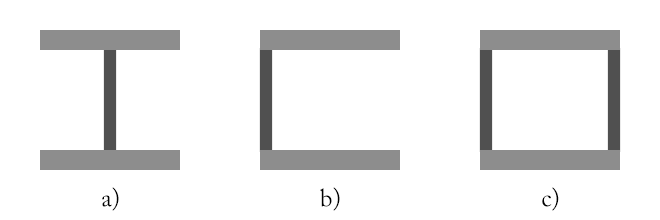
\includegraphics[width=1.0\textwidth]{Bilder/Holmarten.png}
	\caption{Holmarten: a) I-Holm   b) C-Holm    c) Kastenholm}
	\label{fig: Holmarten}
\end{figure}\\ 
\noindent
Das aerodynamische Profil des Flügels wird durch die Schale erreicht. Hierbei wird eine dünne Haut nur an kritischen Stellen mit der Sandwichbauweise oder Rippen verstärkt, um Beulen zu verhindern. Die Schale trägt dabei so gut wie gar nicht die Last des Flügels, jedoch ist sie für die Torsionssteifigkeit entscheidend.
\FloatBarrier